%\documentclass[handout,space,nooutcomes]{ximera}
\documentclass{ximera}

\title{Paying off Debt}

\begin{document}
\begin{abstract}
Here we investigate where your payments go when you pay off debt.
\end{abstract}
\maketitle

When you take out a loan, the amount of the loan is called
\textbf{principal}.  For most loans, interest is calculated monthly,
based on an \textbf{annual interest rate}, and based on the remaining
balance.  When you make a payment, your payment first offsets the
accumulated interest and then is applied to principal, in order to
calculate the \textbf{remaining principal balance}.  The loan is paid
back in full when the remaining principal balance is reduced to zero.

\begin{question}%[1in]
Suppose you borrow $\$5,000$ and agree to pay it back in equal annual
payments over $5$ years.  Interest is calculated at $7\%$,
compounded annually. 

%% Without making any calculations, make a guess at what the annual payment should be.  
%% \begin{freeResponse}
%% \end{freeResponse}
%% \end{question}

%% \begin{question}[0in]
We will approach this problem numerically.  Use a guess of $\$1250$
for your annual payment to complete the table below. Round
all answers to the nearest cent.
%(Do this work on paper, offline.  In Ximera, enter just the last row of your table.)  
\[
  \begin{array}{|c|c|c|c|c|}
    \hline
    \text{Year} & \text{Interest}             & \text{Balance with Interest} & \text{Payment}    & \text{Remaining Principal Balance}\\ \hline
    0  & \$ 0               & ---                   & \$ 0     & \$ 5000 \\ \hline
    1  & \$ \answer{350}    & \$ \answer{5350}    & \$ 1250  & \$ \answer{4100} \\ \hline
    2  & \$ \answer{287}    & \$ \answer{4387}    & \$ 1250  & \$ \answer{3137} \\ \hline
    3  & \$ \answer{219.59} & \$ \answer{3356.59} & \$ 1250  & \$ \answer{2106.59} \\ \hline
    4  & \$ \answer{147.46} & \$ \answer{2254.05} & \$ 1250  & \$ \answer{1004.05} \\ \hline
    5  & \$ \answer{70.28}  & \$ \answer{1074.33} & \$ 1250  & \$ \answer{-175.67} \\ \hline
  \end{array}
\]

%% \begin{image}
%% 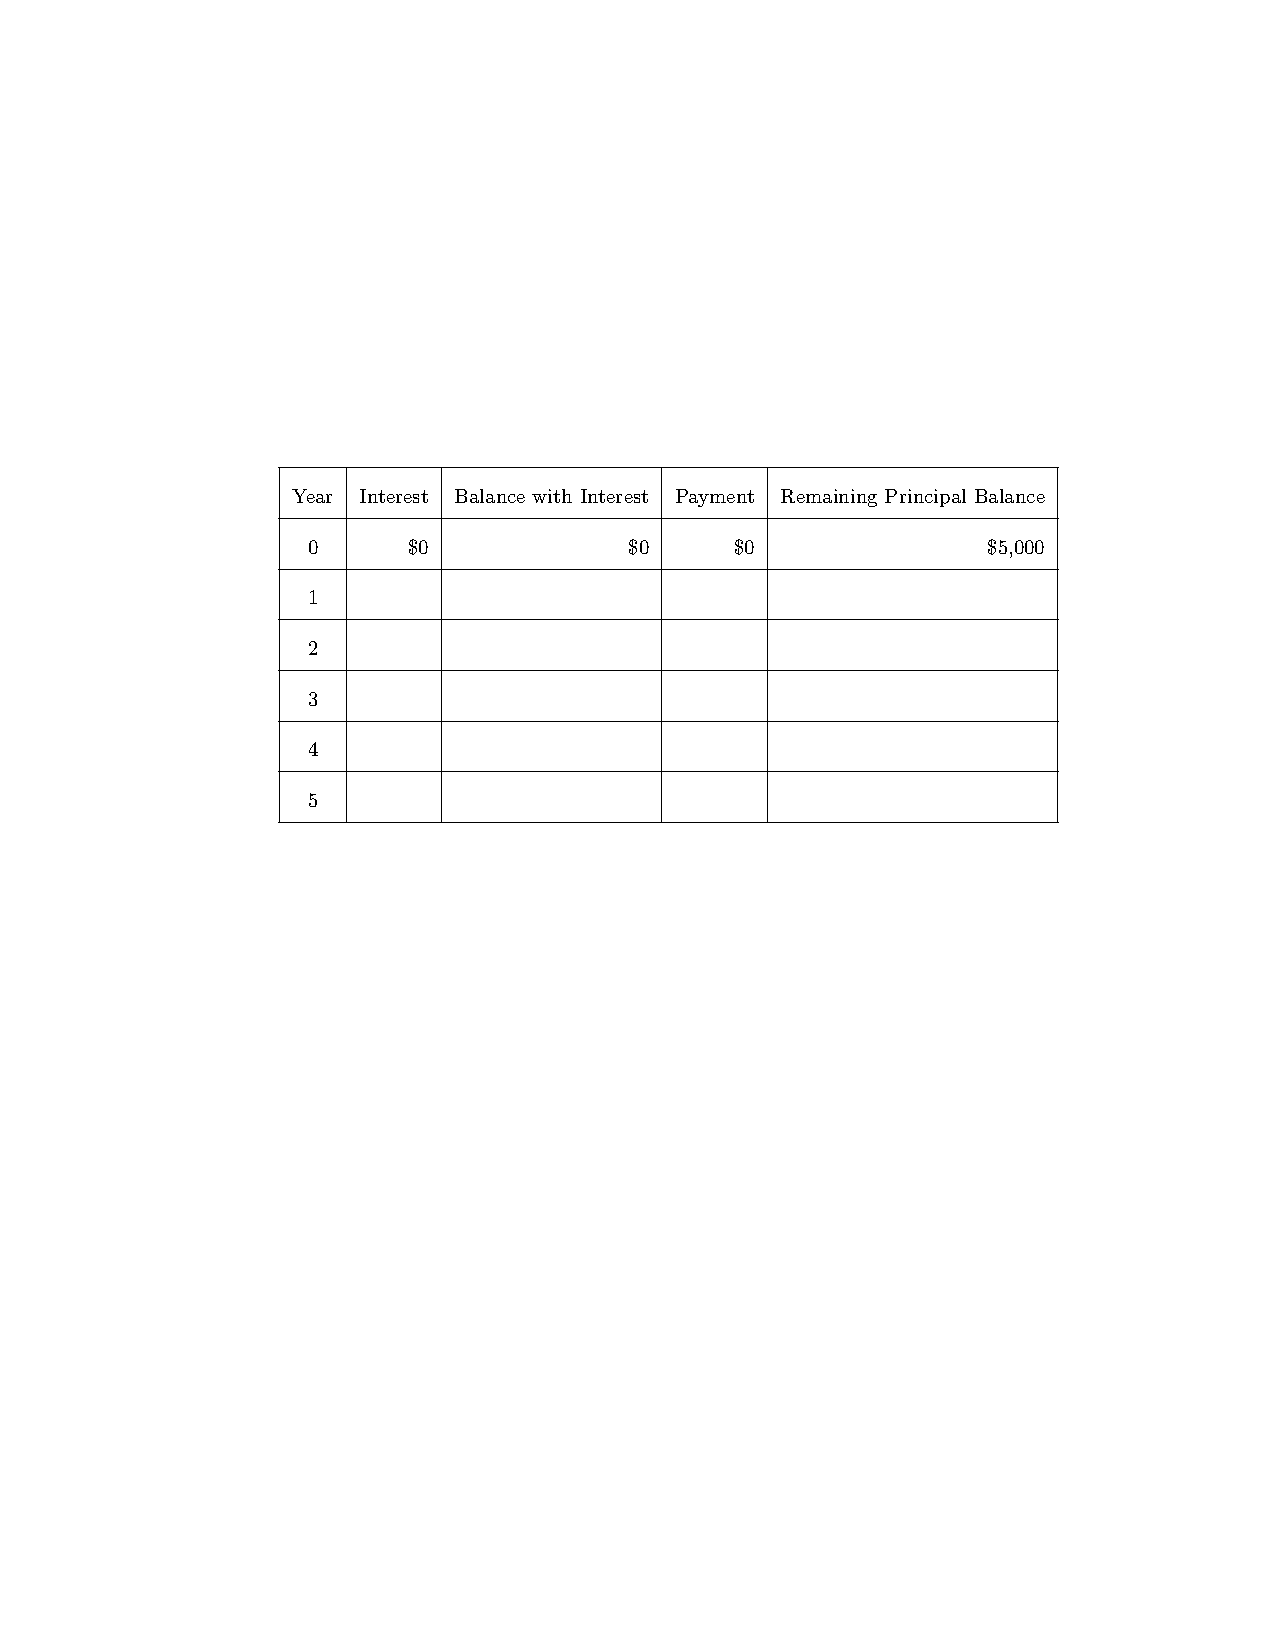
\includegraphics{payingOffDebtTableGraphic.pdf}
%% \end{image}
%% \begin{freeResponse}
%% \end{freeResponse}
\end{question}

\begin{question}
Based on your table, was your guess is too low, too high, or just
right?
\begin{multipleChoice}
  \choice{Too low}
  \choice[correct]{Too high}
  \choice{Just right}
\end{multipleChoice}

\end{question}

\begin{question}%[0in]
  %Complete the table again for other possible payment amounts until
  %you have found the ``best'' annual payment.  %(In Ximera, enter just
  %the last row of your table.)

  Complete the table again for a payment
  of $\$1219.45$.  Round all answers to the nearest cent.
  \[
  \begin{array}{|c|c|c|c|c|}
    \hline
    \text{Year} & \text{Interest}             & \text{Balance with Interest} & \text{Payment}    & \text{Remaining Principal Balance}\\ \hline
    0  & \$ 0               & ---                   & \$ 0        & \$ 5000 \\ \hline
    1  & \$ \answer{350}    & \$ \answer{5350}    & \$ 1219.45  & \$ \answer{4130.55} \\ \hline
    2  & \$ \answer{289.14} & \$ \answer{4419.69} & \$ 1219.45  & \$ \answer{3200.24} \\ \hline
    3  & \$ \answer{224.02} & \$ \answer{3424.26} & \$ 1219.45  & \$ \answer{2204.81} \\ \hline
    4  & \$ \answer{154.34} & \$ \answer{2359.15} & \$ 1219.45  & \$ \answer{1139.70} \\ \hline
    5  & \$ \answer{79.78}  & \$ \answer{1219.48} & \$ 1219.45  & \$ \answer{0.03} \\ \hline
    \end{array}
  \]

%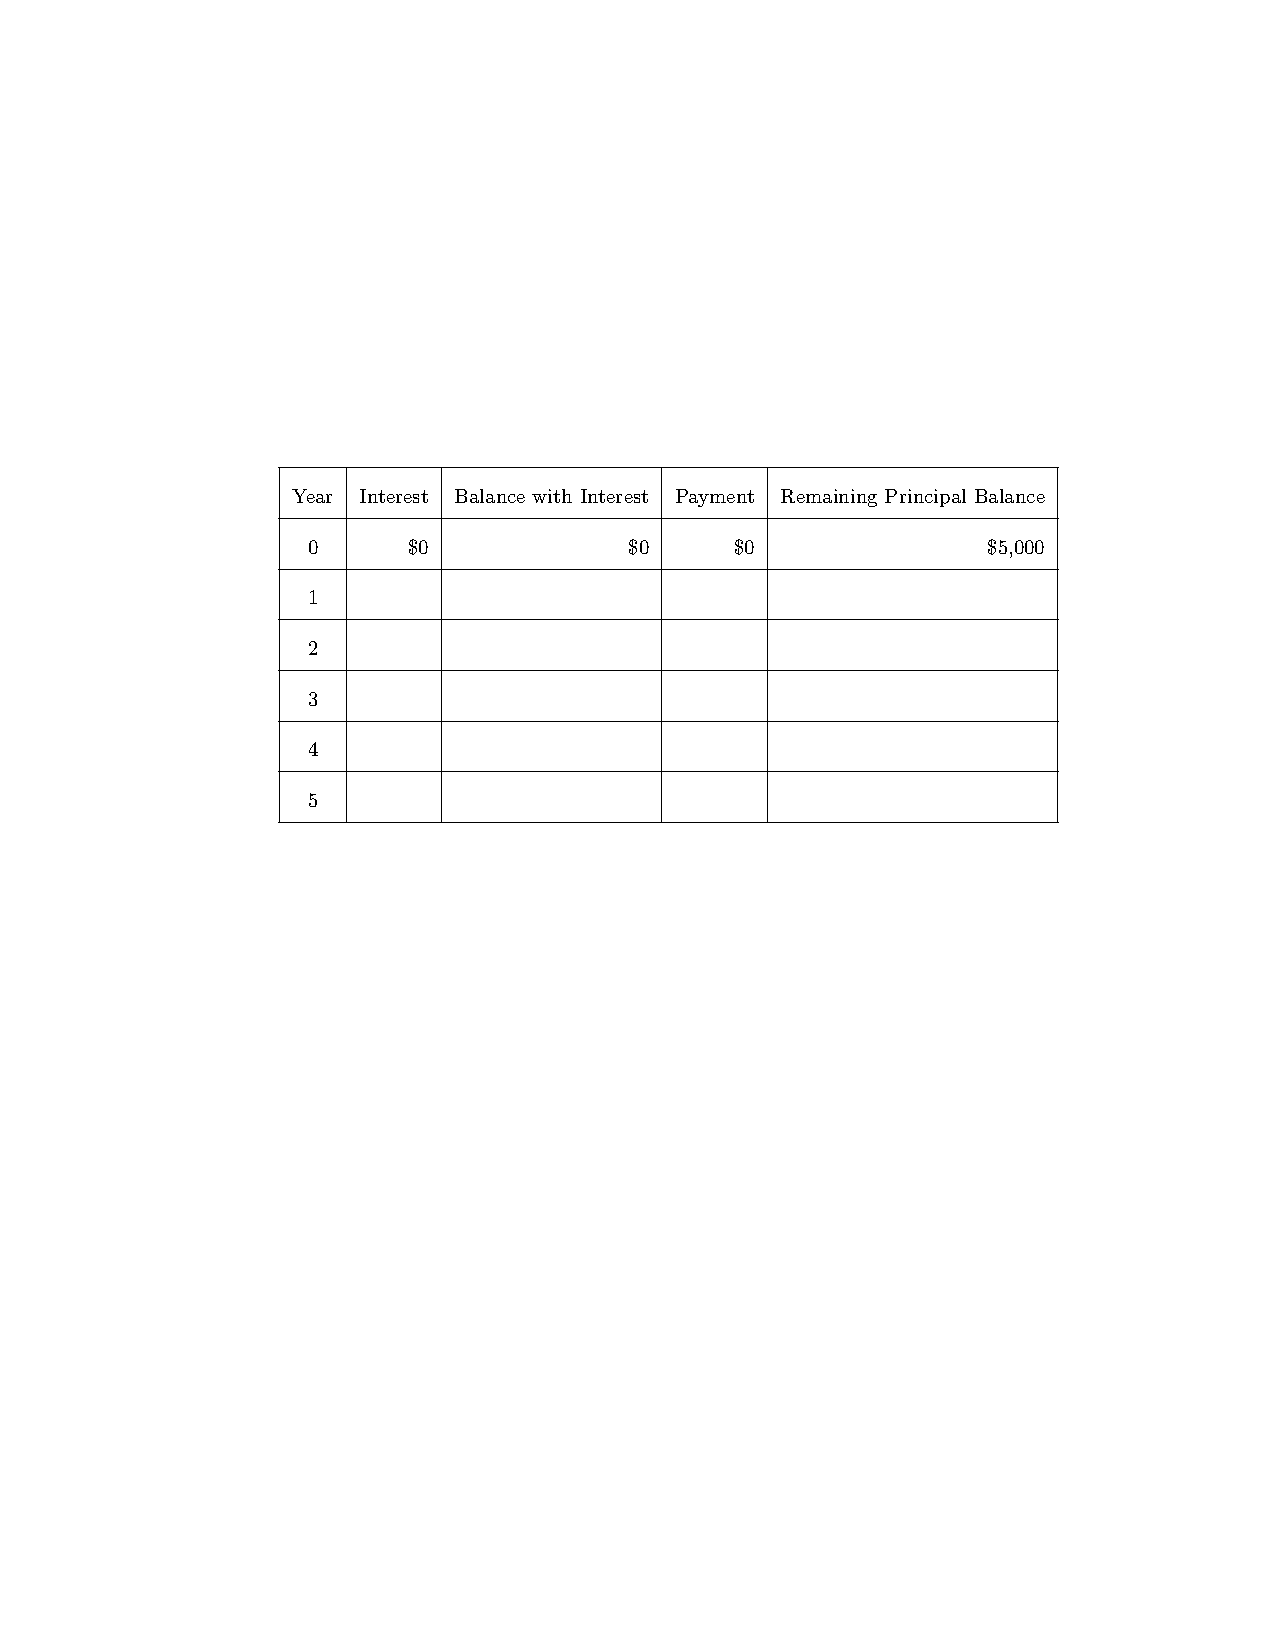
\includegraphics{payingOffDebtTableGraphic.pdf}
\end{question}

\begin{question}
Using your best annual payment, how much interest would you pay in total over the $5$ years? 
\begin{prompt}
  You would pay \$ $\answer{1097.28}$.
\end{prompt}
\end{question}

%% \begin{question}[.5in]
%% Complete the table again, this time with a beginning principal of $P$, an interest rate of $r$,
%% and a payment amount of $x$.  Hint: It helps to collect factors of $(1+r)$.

%% Then write an equation that must be true if $x$ is the correct
%% payment amount.   %(In Ximera, enter just the equation.)

%% 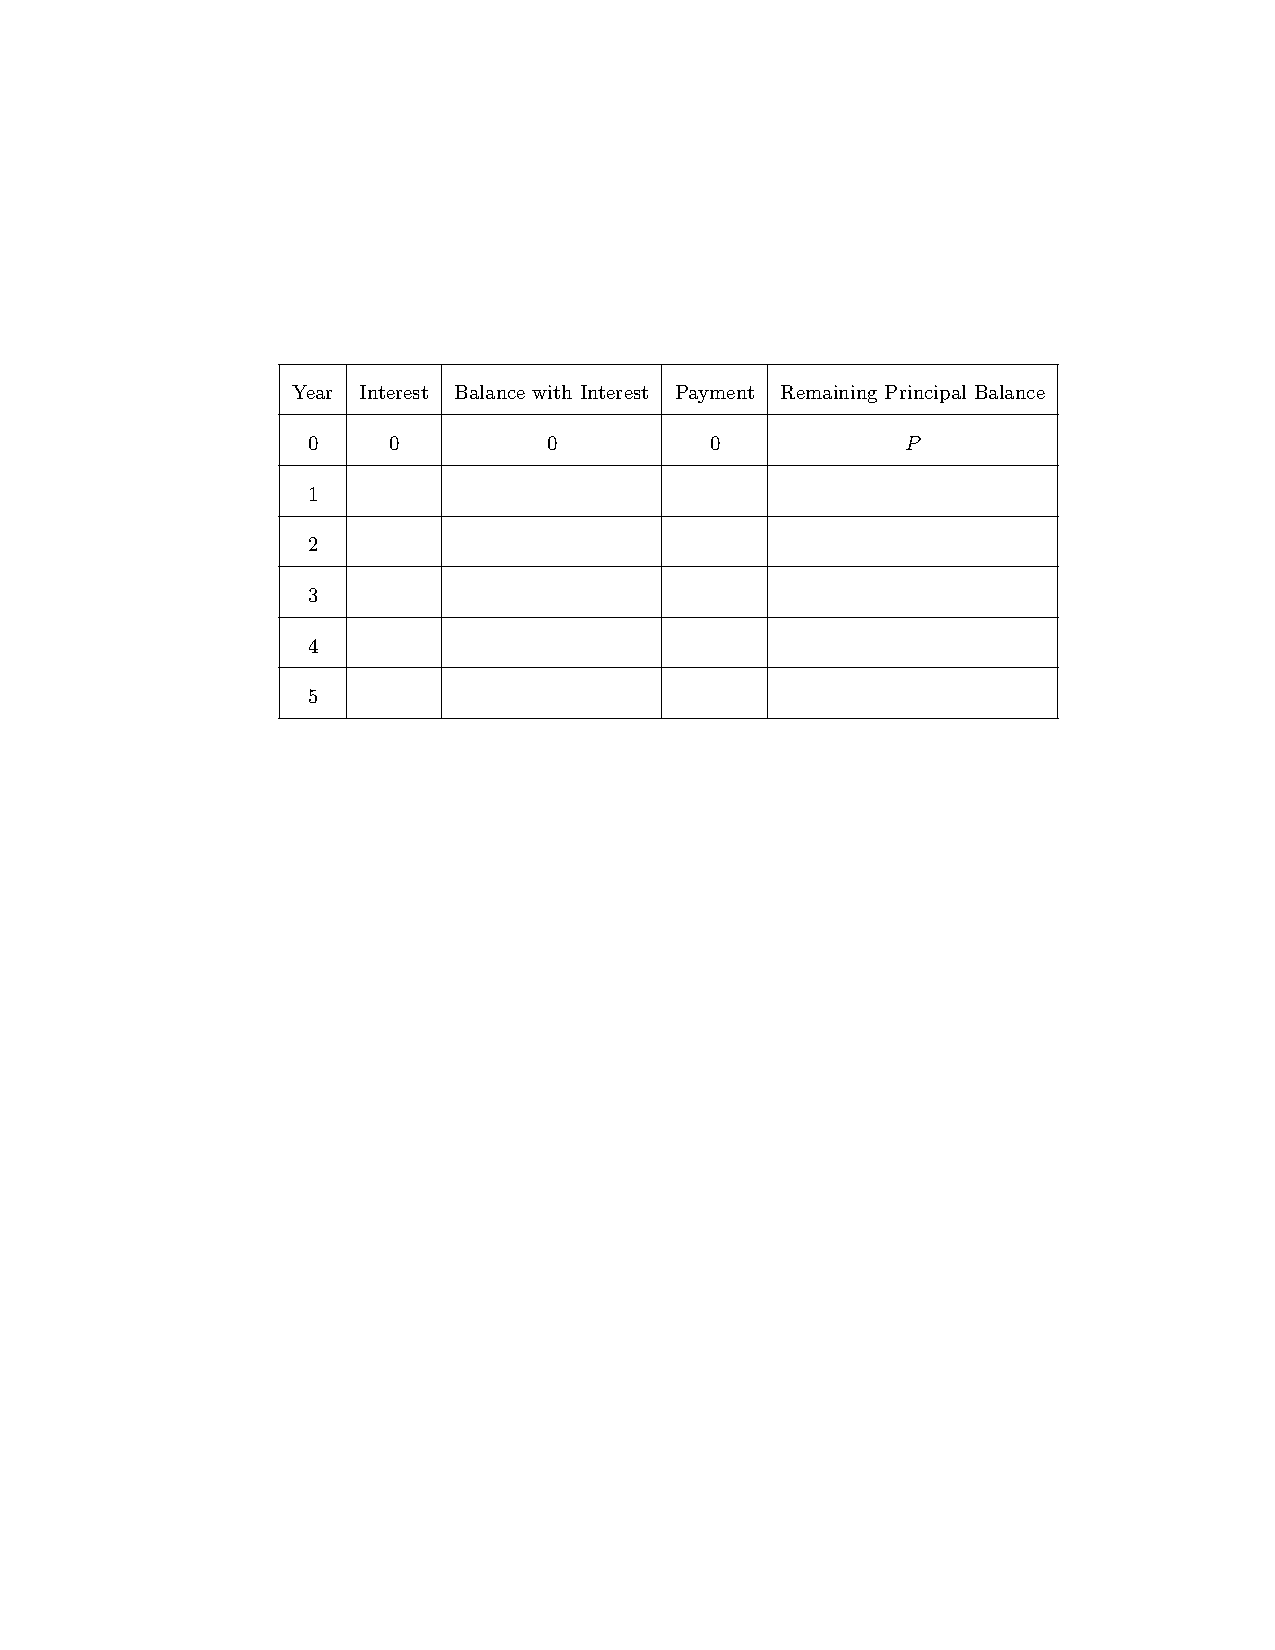
\includegraphics{payingOffDebtTableGraphic2.pdf}

%% \begin{freeResponse}
%% \end{freeResponse}
%% \end{question}

%% \begin{question}
%% What is your next question?   
%% \begin{freeResponse}
%% \end{freeResponse}
%% \end{question}


%\begin{question}
%Some students notice that the equation above includes a geometric series.  Write the geometric series here.
%\begin{freeResponse}
%\end{freeResponse}
%\end{question}
%
%\begin{question}
%How do you know this is a series?  How do you know this is a geometric series?   
%\begin{freeResponse}
%\end{freeResponse}
%\end{question}
%
%\begin{question}
%Call the geometric series $S$, and note that if you multiply $S$ by $1.07$, the ``common ratio,'' you get another geometric series with many of the same terms.  Use these observations to find the sum of the series.   
%\begin{freeResponse}
%\end{freeResponse}
%\end{question}


\end{document}
